\documentclass[11pt,oneside]{scrbook}
\usepackage[a4paper,margin=2.4cm,marginparwidth=1.8cm,marginparsep=0.4cm]{geometry}
\usepackage{../common/rlstudy}
\usepackage[ruled,vlined]{algorithm2e}

\title{{\color{rlblue}\textbf{Week 16} \\ \Huge Model-Based RL: Dreamer, MuZero, and Latent World Models}}
\author{STUDY-RL --- a self-paced Deep RL curriculum}
\date{\today}

\begin{document}
\maketitle
\tableofcontents
\newpage

\chapter*{Learning objectives}
\addcontentsline{toc}{chapter}{Learning objectives}

% Teaching companion: a small example before the full lecture.
\noindent\textbf{Study companion.} Read \texttt{teaching\_guide.md} in this
folder for step-by-step examples, an analogy with its limits, and self-checks.
Then use \texttt{workbook.ipynb} to implement and vary the calculations.
\par\medskip

\begin{keyidea}
After this week you will:
\begin{enumerate}
  \item Distinguish PETS-style ``ensemble dynamics + MPC'' from latent world models like Dreamer.
  \item Derive the Dreamer ELBO: reconstruction + reward + continue + KL between posterior and prior over the stochastic latent.
  \item Derive the actor-critic-in-imagination update with $\lambda$-returns.
  \item Implement a tiny RSSM and train an actor in imagination on CartPole; visualise imagined vs.\ real rollouts.
  \item Summarise MuZero / EfficientZero / TD-MPC2 / DIAMOND and place them on the planning--learning axis.
  \item Articulate where a learned world model is safer (and where it is not) than a model-free policy.
\end{enumerate}
\end{keyidea}

\chapter{Motivation \& intuition}

A world model is a learned simulator. Once you have one, you can generate as many synthetic experiences as you want --- this is sample-efficiency by hallucination.\marginnote{Hallucination here is desirable. We feed it back to the learner; the world doesn't have to consent.} The model-based family ranges from PETS (probabilistic ensembles + MPC) through Dreamer (latent world model with imagination-trained actor) to MuZero (tree search on a learned latent).

\begin{intuition}
Model-free RL is like learning to drive by trial and error on real streets. Model-based RL is building a driving simulator from your experience and then practising any manoeuvre you like inside the simulator. Dreamer is special because the simulator is \emph{abstract} --- it does not need to look like the world, only act like it under reward.
\end{intuition}

\chapter{Mathematical formulation}

\section{The Recurrent State-Space Model (RSSM)}

\begin{definition}[RSSM]
At each step $t$, the agent maintains:
\begin{itemize}
  \item a deterministic recurrent state $h_t = \mathrm{GRU}(h_{t-1}, [s_{t-1}, a_{t-1}])$,
  \item a stochastic latent $s_t \sim p(s_t \mid h_t)$ called the \emph{prior},
  \item posterior $s_t \sim q(s_t \mid h_t, o_t)$ when an observation $o_t$ is available.
\end{itemize}
\end{definition}

The model emits:
\[
  o_t \sim p(o_t \mid h_t, s_t), \quad r_t \sim p(r_t \mid h_t, s_t),\quad c_t \sim p(c_t \mid h_t, s_t),
\]
where $c_t \in \{0, 1\}$ is the continue flag.

\section{Dreamer world-model ELBO}

\begin{theorem}[Dreamer world-model objective]
Index reward and continuation by arrival: action $a_{t-1}$ leads to $(o_t,r_t,c_t)$. For $\tau=(o_{1:T},a_{0:T-1},r_{1:T},c_{1:T})$, conditioning on the actions, the negative ELBO at $\beta=1$ is
\[
\begin{aligned}
  -\mathcal{L}(\theta, \phi)
  ={}& \sum_{t=1}^{T} \E_{q_\phi}\bigl[
    \underbrace{-\log p_\theta(o_t \mid h_t, s_t)}_{\text{reconstruction}}
    -\log p_\theta(r_t\mid h_t,s_t)\\
    &\hspace{4.5cm} -\log p_\theta(c_t\mid h_t,s_t)\bigr]\\
  &+ \beta \sum_{t=1}^{T} \E_{q_\phi}\bigl[
    \KL(q_\phi(s_t \mid h_t, o_t) \,\|\, p_\theta(s_t \mid h_t))\bigr].
\end{aligned}
\]
\end{theorem}

\begin{proof}[Derivation]
Start from $\log p_\theta(o_{1:T}, r_{1:T}, c_{1:T}\mid a_{0:T-1}) \geq \E_{q_\phi}[\log p_\theta(o, r, c, s) - \log q_\phi(s)]$, factor the joint by the temporal Markov structure of the RSSM, and gather the $-\KL$ terms per timestep. Choosing $\beta\ne1$ reweights this objective and is no longer the standard ELBO identity; Dreamer V2 introduces ``KL balancing'' --- stop-gradients on either side --- to control whose distribution moves.
\end{proof}

\begin{pitfall}
KL balancing controls how strongly the prior and posterior are updated; it is not a universal cure or a mathematical requirement for every RSSM. Posterior collapse can arise from the interaction of KL pressure and the decoder. The project uses free-nats clipping; exercise 5 demonstrates balancing separately.
\end{pitfall}

\section{Actor-critic in imagination}

\begin{definition}[Imagination rollout]
Given a latent state $(h_0, s_0)$ obtained from posterior inference on real data, the
\emph{imagined trajectory} is generated by sampling $a_t \sim \pi_\psi(\cdot \mid h_t, s_t)$,
stepping the prior $s_{t+1} \sim p_\theta(\cdot \mid h_{t+1})$ with
$h_{t+1} = \mathrm{GRU}(h_t, [s_t, a_t])$, and reading off $r_t, c_t$ from the model heads.
\end{definition}

\begin{theorem}[$\lambda$-return for imagined rollouts]
The bootstrap target for the critic is the lambda-return
\[
  G_t^\lambda = r_t + \gamma c_t \bigl[(1 - \lambda) V_\xi(h_{t+1}, s_{t+1}) + \lambda G_{t+1}^\lambda\bigr],
  \qquad G_H^\lambda = V_\xi(h_H, s_H).
\]
\end{theorem}

Actor and critic losses:
\[
  \mathcal{L}_\psi = -\E\!\left[\sum_t \log \pi_\psi(a_t \mid h_t, s_t) \cdot \bigl(G_t^\lambda - V_\xi(h_t, s_t)\bigr)\right],\quad
  \mathcal{L}_\xi = \E\!\left[\sum_t (V_\xi(h_t, s_t) - G_t^\lambda)^2\right].
\]

The advantage is the lambda-return target minus the current-state value baseline. In the REINFORCE loss, stop gradients through that advantage; the critic targets are detached too. Dreamer V2/V3 replace the REINFORCE actor by a path-derivative one when actions are continuous; for discrete actions we use straight-through with Gumbel-softmax or REINFORCE as above.

\section{PETS and MBPO --- the alternative}

\textbf{PETS} fits an ensemble of probabilistic dynamics models and plans by sampling
trajectories under the model (CEM in action space). \textbf{MBPO} interleaves
short-horizon model rollouts with real data in an SAC-style buffer:
$D_{\mathrm{train}} = D_{\mathrm{real}} \cup D_{\mathrm{model}}$. The MBPO theorem bounds the
policy-performance gap using assumptions on rewards, model error, policy shift, and rollout horizon. State-distribution errors can accumulate and affect all later rewards, so total return error is not generally just one-step error times horizon. Short rollouts branched from real data reduce this accumulation.

\section{MuZero, EfficientZero V2, TD-MPC2}

MuZero learns three networks --- representation $h$, dynamics $g$, prediction $f$
(value + policy) --- jointly via MCTS-derived training targets. Crucially the model is
\emph{not} trained to reconstruct observations; it is trained so the values and policies
at any imagined state match the MCTS roots and chosen actions. EfficientZero V2 adds
data augmentation and a self-supervised consistency loss, achieving DQN-level Atari with
$\sim$2 hours of game time. TD-MPC2 combines a learned latent model with MPC at deployment
and TD-learning of a value function, scaling to large multi-task settings.

\section{DIAMOND --- diffusion world models}

DIAMOND (Alonso 2024) replaces the deterministic decoder with a denoising diffusion model
over pixel frames, conditioned on a small encoder feature. The denoiser is the world model;
the policy is trained from the denoised rollouts as in Dreamer. The trade-off: very high
sample fidelity, very high compute cost.

\chapter{Algorithms}

\begin{algorithm}[H]
\caption{Dreamer-lite}
\KwIn{Replay buffer $\mathcal{D}$, RSSM $\theta$, actor $\psi$, critic $\xi$.}
\For{iteration = 1, ..., N}{
  Collect episodes with the actor (epsilon-greedy)\;
  \For{world-model step = 1, ..., $W$}{
    Sample chunks; posterior-roll the RSSM; minimise the ELBO\;
  }
  \For{behaviour step = 1, ..., $B$}{
    Posterior-roll to a batch of latent states; imagine $H$ steps under $\pi_\psi$\;
    Compute $G^\lambda$; backprop actor (REINFORCE) and critic (MSE)\;
  }
  Evaluate\;
}
\end{algorithm}

\textbf{Complexity:} dominated by the RSSM forward pass: $O(L \cdot d^2)$ per chunk of length
$L$ and hidden width $d$. Imagination adds $O(H \cdot d^2)$ per behaviour step.

\section{Worked numerical example}

Take a 2-step CartPole-like rollout. Suppose the actor outputs $\pi = (0.7, 0.3)$ at
$h_0, s_0$. It samples $a_0 = 0$, the prior produces $s_1$ with $r_0 = 1$, $c_0 = 0.99$.
At $h_1, s_1$ the actor samples $a_1 = 1$ with $\log \pi = -1.2$, the prior gives
$r_1 = 1$, $c_1 = 0.98$. Critic outputs $V_0 = 5, V_1 = 4, V_2 = 3$. With
$\gamma = 0.99, \lambda = 0.95$,
\begin{align*}
G_1^\lambda &= 1 + 0.99 \cdot 0.98 \cdot [0.05 \cdot 3 + 0.95 \cdot 3] = 1 + 0.9702 \cdot 3 = 3.91, \\
G_0^\lambda &= 1 + 0.99 \cdot 0.99 \cdot [0.05 \cdot 4 + 0.95 \cdot 3.91] = 1 + 0.9801 \cdot (0.2 + 3.715) = 4.84.
\end{align*}
The sampled actor loss term at $t=0$ is $-\log \pi(a_0=0) \cdot (G_0^\lambda - V_0) = -\log 0.7 \cdot (4.84 - 5) = -(-0.357) \cdot (-0.16) = -0.057$ --- a negative loss contribution, not the gradient itself. Differentiating with the advantage detached gives a push \emph{away} from $a_0$ because the realised return was slightly worse than the baseline.

\chapter{Implementation walkthrough}

\begin{codebox}
\begin{minted}{python}
# World-model step: posterior roll, four-component loss.
state = rssm.initial(B, device)
for t in range(L):
    state, prior_mu, prior_std, post_mu, post_std, recon, r_pred, c_pred = \
        rssm.observe_step(state, A_oh[:, t], O[:, t+1])
    recon_loss += ((recon - O[:, t+1])**2).sum(-1).mean()
    rew_loss   += ((r_pred - R[:, t])**2).mean()
    cont_loss  += F.binary_cross_entropy(c_pred, C[:, t])
    kl = kl_gaussian(post_mu, post_std, prior_mu, prior_std)
    kl_loss   += torch.clamp(kl, min=free_nats).mean()
\end{minted}
\end{codebox}

The behaviour step then opens a fresh imagination from each posterior state, computes
the lambda-return, and updates actor + critic.

\chapter{Empirical results}

\begin{figure}[h]
\centering
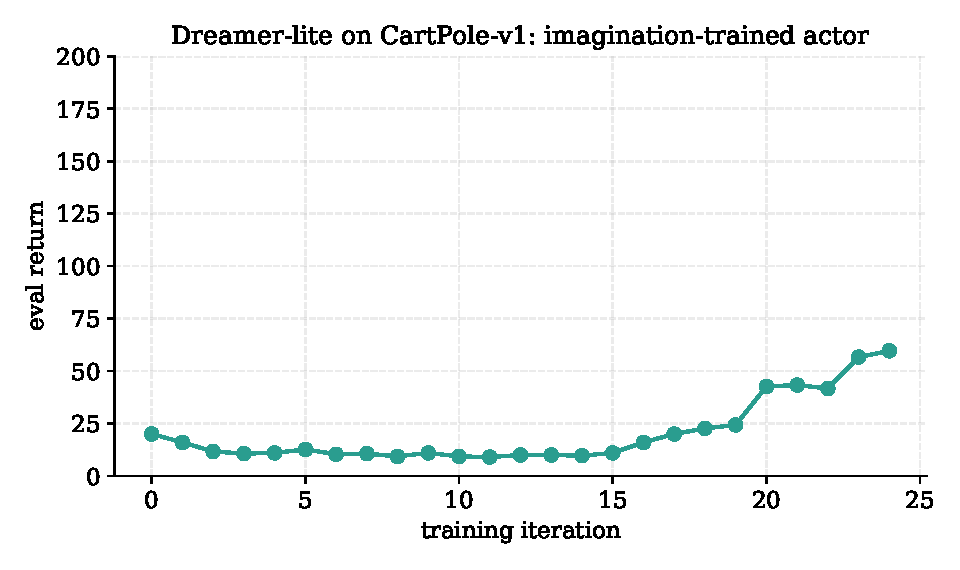
\includegraphics[width=0.85\textwidth]{figs/fig_dreamer_curve.pdf}
\caption{Dreamer-lite on CartPole-v1, 25 iterations $\approx$ 15--30s on a single GPU.
Mean evaluation return ramps from $\sim$20 (random) to $\sim$60 (the cap of 200 we use to
keep tests fast). Full Dreamer reaches the maximum of 500.}
\end{figure}

\begin{figure}[h]
\centering
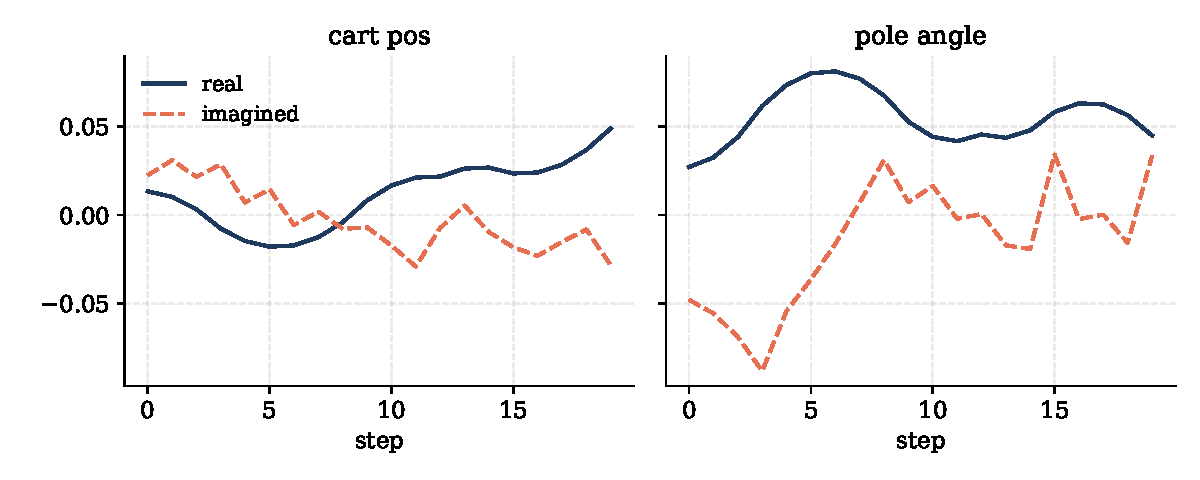
\includegraphics[width=\textwidth]{figs/fig_imagined_vs_real.pdf}
\caption{Imagined trajectory under the learned RSSM (dashed) vs.\ the real environment
trajectory (solid) under the same actor. The world model captures the qualitative
dynamics but accumulates error over time --- the canonical model-based-RL tension.}
\end{figure}

\begin{safetyangle}
\textbf{World-model deployment failure modes.}
\begin{enumerate}
  \item \textbf{Reward hacking the model.} An imagination-trained actor will exploit
        any flaw in the world model: predicting infinite reward for an unreachable
        state, exploiting the continue head to ``stay alive forever''.
  \item \textbf{Distributional brittleness.} The latent dynamics are accurate only
        on states near the training distribution. Long-horizon imagination diverges,
        so a policy purely improved on long imagined rollouts may collapse on real
        data.
  \item \textbf{Mitigations.} Cap imagination horizon ($H = 15$ in Dreamer V3);
        use a *value-equivalence* objective (MuZero) when reconstruction is not
        the deployment signal; mix imagined data with a steady stream of real
        experience.
\end{enumerate}
Citations: \textsc{Hafner et al.\ 2023, ``Mastering Diverse Domains''}; \textsc{Schrittwieser et al.\ 2020, ``MuZero''}.
\end{safetyangle}

\begin{matching}
\textbf{World models for recruitment matching.} The ATS analogue is a latent model of
``candidate trajectory dynamics'': given a stage-history of decisions, the model
predicts the next state distribution under different recruiter actions. A Dreamer-style
training loop would let the system simulate the consequences of hypothetical recruiter
decisions before taking them --- crucial for a domain where each ``rollout'' on a real
candidate is expensive, slow, and ethically loaded. The safety angle then becomes:
the world model must be \emph{audited} for fairness in its imagined dynamics, not just
its terminal outcomes.
\end{matching}

\chapter{Exercises}

See \texttt{workbook.ipynb}.
\begin{itemize}
  \item \textbf{Ex.\ 1 ($\star$)} Closed-form KL between diagonal Gaussians.
  \item \textbf{Ex.\ 2 ($\star$)} Lambda-return computation.
  \item \textbf{Ex.\ 3 ($\star\star$)} Build a tiny RSSM and imagine a step.
  \item \textbf{Ex.\ 4 ($\star\star$)} Run Dreamer-lite for 12 iterations.
  \item \textbf{Ex.\ 5 ($\star\star\star$)} KL-balancing trick (Dreamer V2).
  \item \textbf{Ex.\ 6 ($\star\star$)} Compare imagined and real rollouts.
  \item \textbf{Ex.\ 7 ($\star\star$)} World-model loss components.
  \item \textbf{Ex.\ 8 ($\star\star\star$, meaningful objective)} Recruitment world-model essay.
\end{itemize}

\chapter{Further reading}

See \texttt{extended\_reading.pdf} for Chua et al.\ 2018 (PETS), Janner et al.\ 2019
(MBPO), Hafner et al.\ 2023 (Dreamer V3), Schrittwieser et al.\ 2020 (MuZero), and
Alonso et al.\ 2024 (DIAMOND). Sourced from \texttt{research/offline\_modelbased\_sota.md}
(Track B).

\end{document}
